\documentclass{article}
\usepackage[utf8]{inputenc}
\usepackage[english]{babel}
\usepackage[]{amsthm} 
\usepackage[]{amssymb} 
\usepackage{amsmath}
\usepackage{graphicx}
\usepackage{hyperref}
\usepackage{mathtools}
\usepackage[thinc]{esdiff}
\usepackage[dvipsnames]{xcolor}
\usepackage{float}
\usepackage{listings}
\graphicspath{ {./HW4_img/} }

\title{ADSP: HW4}
\author{Lo Chun, Chou \\ R13922136}
\date\today


\begin{document}
\setlength{\parindent}{0pt}
\maketitle 

\section*{(1)}

The following image is the comparison between the 4:2:0 compressed image and the reconstructed image, 
and the PSNR value is shown in the title:

\begin{figure}[H]
    \centering
    
\includegraphics[width=\textwidth]{problem_1/comparison.png}
\end{figure}

Since we need to do reconstruction, instead of directly finding a 4:2:0 compressed image,
I first use an arbitrary image, compress it, and then reconstruct it.
\bigskip

For the code, please refer to the attached file on NTUCOOL.

\section*{(2)}

\subsection*{(a)}

The two reasons why DCT is used instead of DFT for transformation are:

\begin{itemize}
    \item DCT is a real-valued transform, while DFT is a complex-valued transform, 
    hence by using DCT, we do not need to deal with imaginary part, 
    which would reduce the complexity of calculation, and requires less memory for storage.
    \item From the lecture note: "ADSP\_Write4.pdf", p.296, 
    we can see that DCT has more energy concentration at low frequencies compared to DFT,
    therefore, more of the data in the higher frequencies can be discarded,
    which would have better compression performance.
\end{itemize}

\subsection*{(b)}

Two reasons why the input image is separated into 8x8 blocks before using DCT are:

\begin{itemize}
    \item We can \underline{save memory} by using 8x8 blocks, 
    because each of the point in the image needed to be saved in the memory during calculation,
    so if we only use 8x8 block, we only need to save 64 points in the memory at once,
    which would reduce the usage of memory.
    \item Separating the image into 8x8 blocks would \underline{reduce the complexity} of the calculation,
    since for $M \times N$ point DCT, its complexity is $\theta(MN)$. 
\end{itemize}


\section*{(3)}

\subsection*{(a)}

The three conditions when two images look similar but the NRMSE is large are:

\begin{itemize}
    \item If we \underline{increase brightness} of an image and calculate the NRMSE,
    the resulting value would be large.
    \bigskip

    For example, from the images in lecture note: "ADSP\_Write4.pdf", p.302,
    if we multiply the original image by $0.5$, and add with $255.5 \times 0.5$,
    for the pixels that originally have value $0$, after the transformation, would have value $127.75$,
    which would give great increase to the NRMSE.
    \item If we calculate NRMSE for a photo and its \underline{negative} version, the NRMSE value would be large. 
    (Example in "ADSP\_Write4.pdf", p.306)
    \item If we calculate NRMSE for a photo and a \underline{photo with same shape but different intensity}, the NRMSE value would be large.
    (Example in "ADSP\_Write4.pdf", p.307)
\end{itemize}

\subsection*{(b)}

The two conditions where two vocal signals sound similar but the NRMSE is large are:

\begin{itemize}
    \item If the \underline{phase is different}, even though the two signals have similar frequency, 
    their NRMSE could be large. In the example during lecture, the NRMSE could be even greater than $1$, 
    which ($1$) represents comparing a signal to another signal with all zeros.
    \item Even when two signals are similar, if there's noise in the background, the NRMSE value would be large.
\end{itemize}

\section*{(4)}

We're given the following:

\begin{align*}
    P(x = n) = (1 - e^{-\lambda}) e^{-\lambda n}, \quad \text{for } n = 0, 1, \cdots, 5000, \quad \text{where } \lambda = 0.015
\end{align*}

Also, we suppose $length(x) = 50000$.

\subsection*{(i)}

When using the Huffman code, 
we have the formula in lecture note: "ADSP\_Write4.pdf", p.326:

\begin{figure}[H]
    \centering
    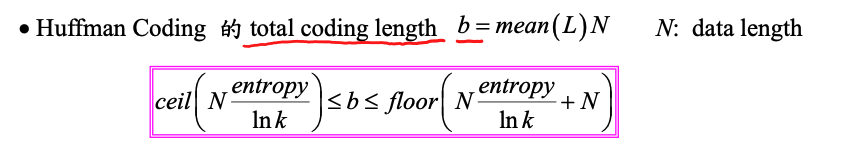
\includegraphics[width=0.8\textwidth]{HW4_img/4_huffman_total_coding_length}
\end{figure}

% \begin{align*}
%     \text{mean}(L) = \sum_{j=1}^{J} P(S_j) L(S_j)
% \end{align*}

% where $P(S_j)$ is the probability of the symbol $S_j$, 
% and $L(S_j)$ is the coding length of the symbol $S_j$.

% \bigskip

% \begin{align*}
%     \text{mean}(L) = \sum_{i=0}^{5000} P(x = i) \log_2 \frac{1}{P(x = i)}
% \end{align*}

Thus, we first calculate the entropy by the formula from lecture note: "ADSP\_Write4.pdf", p.325:

\begin{figure}[H]
    \centering
    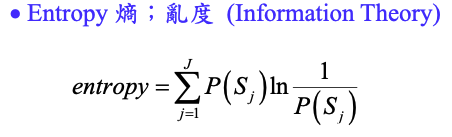
\includegraphics[width=0.7\textwidth]{HW4_img/4_entropy}
\end{figure}

using the scipy library in python, we would calculate the entropy and the range of total coding length:

\begin{align*}
    ceil(50000 \times \frac{\text{entropy (nats)}}{ln 2}) \leq b \leq floor(50000 \times \frac{\text{entropy (nats)}}{ln 2} + 50000)
\end{align*}

The code is as the following:

\begin{figure}[H]
    \centering
    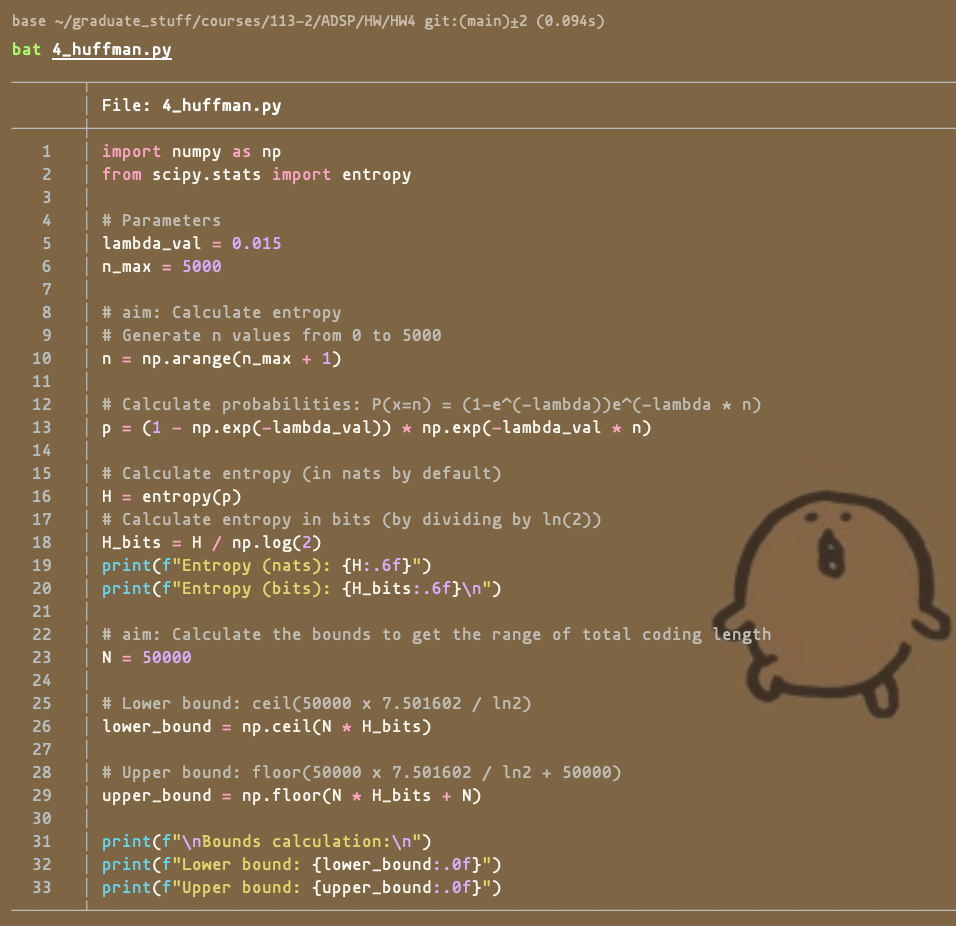
\includegraphics[width=0.9\textwidth]{HW4_img/4_code_huffman.png}
\end{figure}

and the result is:

\begin{figure}[H]
    \centering
    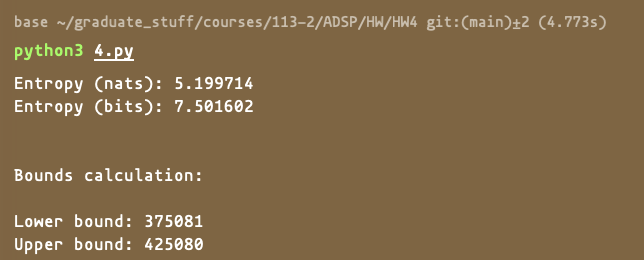
\includegraphics[width=0.7\textwidth]{HW4_img/4_result_huffman.png}
\end{figure}

Thus, the range of total coding length is:

\begin{align*}
    375081 \leq b \leq 425080
\end{align*}


\subsection*{(ii)}

If we use the arithmetic code, the range of total coding length is given by the following formula, 
which is from lecture note: "ADSP\_Write4.pdf", p.338:

\begin{figure}[H]
    \centering
    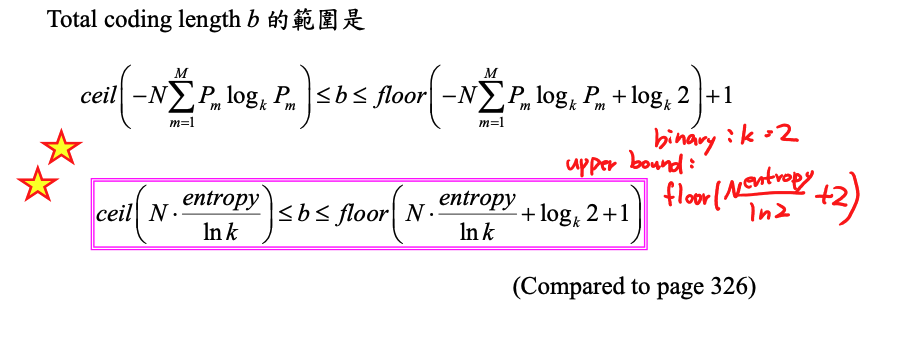
\includegraphics[width=0.8\textwidth]{HW4_img/4_arithmetic_code_total_coding_length.png}
\end{figure}

\bigskip

Similarly, I use the following code to calculate the range of total coding length:

\begin{figure}[H]
    \centering
    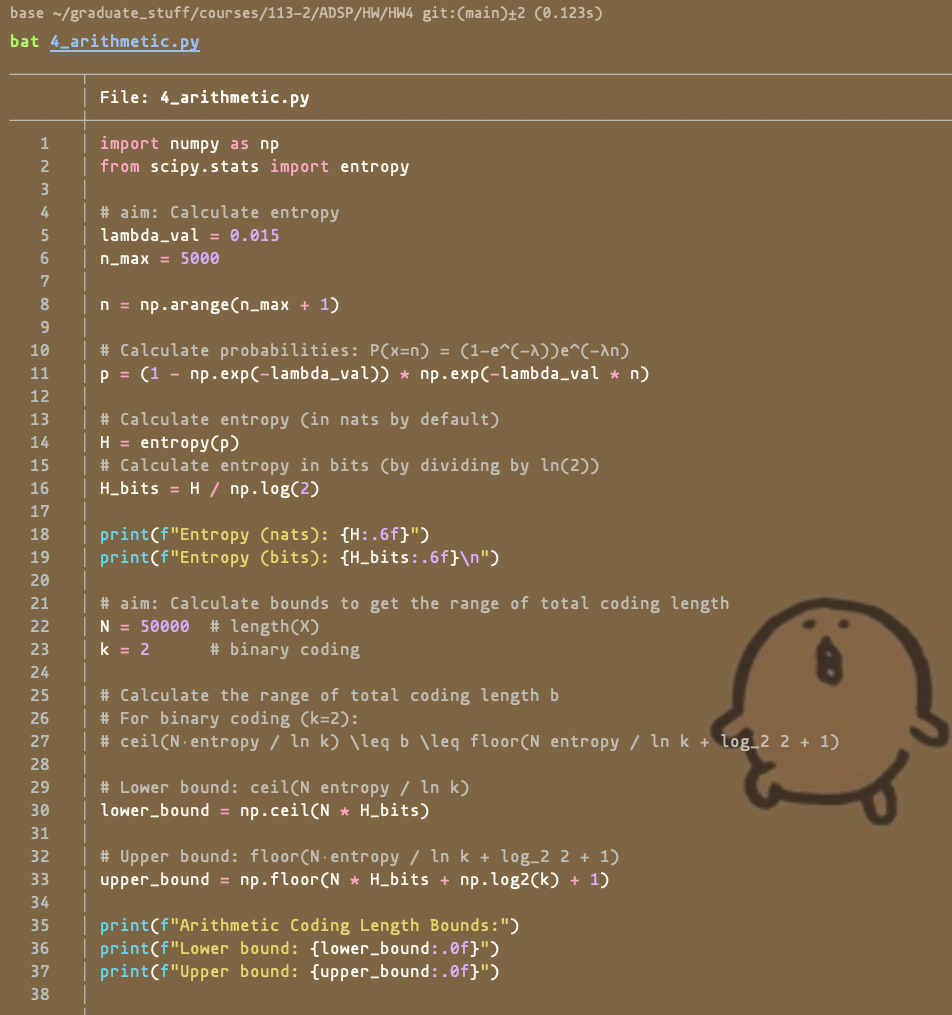
\includegraphics[width=0.9\textwidth]{HW4_img/4_code_arithmetic.png}
\end{figure}

and the result is:

\begin{figure}[H]
    \centering
    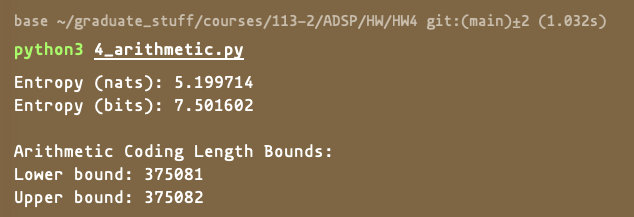
\includegraphics[width=0.7\textwidth]{HW4_img/4_result_arithmetic.png}
\end{figure}

Thus, the range of total coding length is:

\begin{align*}
    375081 \leq b \leq 375082
\end{align*}




\section*{(5)}

Let:

\begin{align*}
    a = 0.7010, \ b = 0.9239, \ c = 0.3827
\end{align*}

Then the given system can be written as:

\begin{align*}
    \begin{bmatrix}
        y_0 \\
        y_1 \\
        y_2 \\
        y_3
    \end{bmatrix} 
    = 
    \begin{bmatrix}
        a & a & a & a \\
        b & c & -c & -b \\
        a & -a & -a & a \\
        c & -b & b & -c
    \end{bmatrix}
    \begin{bmatrix}
        x_0 \\
        x_1 \\
        x_2 \\
        x_3
    \end{bmatrix}
\end{align*}

We can then formulate the system as:

\begin{align*}
    \begin{bmatrix}
        y_0 \\
        y_2 
    \end{bmatrix} 
    &= \begin{bmatrix}
        a & a & a & a \\
        a & -a & -a & a 
    \end{bmatrix}
    \begin{bmatrix}
        x_0 \\
        x_1 \\
        x_2 \\
        x_3
    \end{bmatrix} \\
    &= \begin{bmatrix}
        a & a \\
        a & -a
    \end{bmatrix}
    \begin{bmatrix}
        x_0 + x_3 \\
        x_1 + x_2
    \end{bmatrix}
\end{align*}

which would result in 2 multiplications in this step (by "ADSP\_Write5.pdf", p.354).
\bigskip

Then the other part can be written as:

\begin{align*}
    \begin{bmatrix}
        y_1 \\
        y_3
    \end{bmatrix}
    &= \begin{bmatrix}
        b & c & -c & -b \\
        c & -b & b & -c
    \end{bmatrix}
    \begin{bmatrix}
        x_0 \\
        x_1 \\
        x_2 \\
        x_3
    \end{bmatrix} \\
    &= \begin{bmatrix}
        b & c \\
        c & -b
    \end{bmatrix}
    \begin{bmatrix}
        x_0 - x_3 \\
        x_1 - x_2
    \end{bmatrix}
\end{align*}

which is case 4, and would result in 3 multiplications in this step (by "ADSP\_Write5.pdf", p.360).

\bigskip

In total, we need 5 multiplications.

\section*{(6)}

Consider the case that $\sin \theta = 0$, then the given system (representing the rotation operation):

\begin{align*}
    \begin{bmatrix}
        y_0 \\
        y_1 
    \end{bmatrix}
    = 
    \begin{bmatrix}
        \cos \theta & \sin \theta \\
        -\sin \theta & \cos \theta
    \end{bmatrix}
    \begin{bmatrix}
        x_0 \\
        x_1
    \end{bmatrix}
\end{align*}

would become:

\begin{align*}
    \begin{bmatrix}
        y_0 \\
        y_1 
    \end{bmatrix}
    = 
    \begin{bmatrix}
        \cos \theta & 0 \\
        0 & \cos \theta
    \end{bmatrix}
    \begin{bmatrix}
        x_0 \\
        x_1
    \end{bmatrix}
\end{align*}

Similarly, if $\cos \theta = 0$, then the given system would be:

\begin{align*}
    \begin{bmatrix}
        y_0 \\
        y_1 
    \end{bmatrix}
    = 
    \begin{bmatrix}
        0 & \sin \theta \\
        -\sin \theta & 0
    \end{bmatrix}
    \begin{bmatrix}
        x_0 \\
        x_1
    \end{bmatrix}
\end{align*}

These two cases happen when:

\begin{align*}
    \theta &= \frac{\pi}{2} k, \quad \text{for } \cos \theta = 0 \\
    \theta &= \pi k, \quad \text{for } \sin \theta = 0 \quad \text{where } k \in \mathbb{Z}
\end{align*}
\bigskip

Hence, we can combine these cases and say that when:

\textcolor{Green}{
\begin{align*}
    \theta = \frac{\pi}{2} k, \quad \text{for any } k \in \mathbb{Z}
\end{align*}
}

If $k$ is odd:

\begin{align*}
    \begin{bmatrix}
        y_0 \\
        y_1 
    \end{bmatrix}
    = 
    \begin{bmatrix}
        0 & 1 \\
        -1 & 0
    \end{bmatrix}
    \begin{bmatrix}
        x_0 \\
        x_1 
    \end{bmatrix} \quad \text{or} \quad
    \begin{bmatrix}
        y_0 \\
        y_1 
    \end{bmatrix}
    = 
    \begin{bmatrix}
        0 & -1 \\
        1 & 0
    \end{bmatrix}
    \begin{bmatrix}
        x_0 \\
        x_1 
    \end{bmatrix}
\end{align*}

If $k$ is even:

\begin{align*}
    \begin{bmatrix}
        y_0 \\
        y_1 
    \end{bmatrix}
    = 
    \begin{bmatrix}
        1 & 0 \\
        0 & 1
    \end{bmatrix}
    \begin{bmatrix}
        x_0 \\
        x_1 
    \end{bmatrix} \quad \text{or} \quad
    \begin{bmatrix}
        y_0 \\
        y_1 
    \end{bmatrix}
    = 
    \begin{bmatrix}
        -1 & 0 \\
        0 & -1
    \end{bmatrix}
    \begin{bmatrix}
        x_0 \\
        x_1 
    \end{bmatrix}
\end{align*}

\bigskip

As we could see from the above, we only need two multiplications to multiply with $\pm 1$.
\bigskip

Another situation is that when $|\cos \theta| = |\sin \theta|$, 
which is as the following image:

\begin{figure}[H]
    \centering
    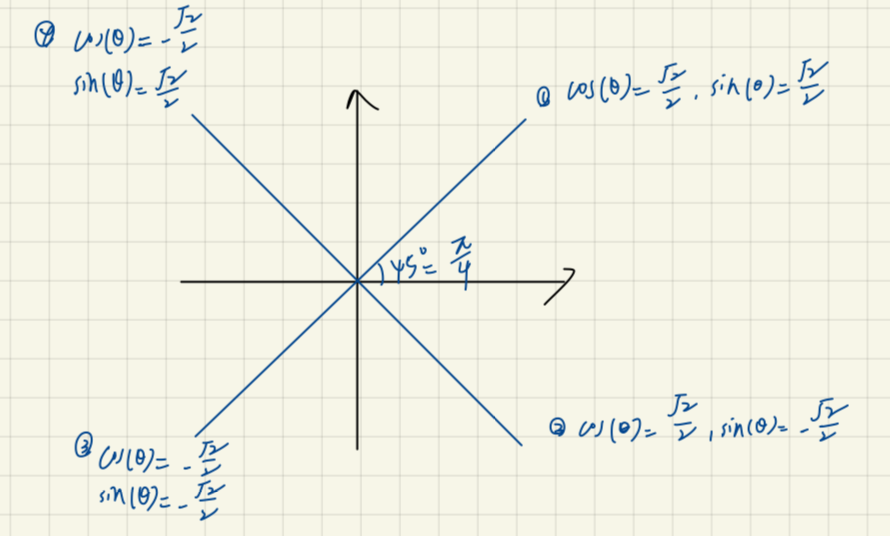
\includegraphics[width=0.7\textwidth]{HW4_img/6.png}
\end{figure}

the given system:

\begin{align*}
    \begin{bmatrix}
        y_0 \\
        y_1 
    \end{bmatrix}
    = 
    \begin{bmatrix}
        \cos \theta & \sin \theta \\
        -\sin \theta & \cos \theta
    \end{bmatrix}
    \begin{bmatrix}
        x_0 \\
        x_1
    \end{bmatrix}
\end{align*}

would become:

\begin{align*}
    \begin{bmatrix}
        y_0 \\
        y_1 
    \end{bmatrix}
    &= 
    \begin{bmatrix}
        \frac{\sqrt{2}}{2} & \frac{\sqrt{2}}{2} \\
        -\frac{\sqrt{2}}{2} & \frac{\sqrt{2}}{2}
    \end{bmatrix}
    \begin{bmatrix}
        x_0 \\
        x_1
    \end{bmatrix} 
    = \begin{bmatrix}
        \frac{\sqrt{2}}{2} (x_0 + x_1) \\
        -\frac{\sqrt{2}}{2} (x_0 + x_1)
    \end{bmatrix}
    \qquad \text{or} \qquad \\
    &= 
    \begin{bmatrix}
        \frac{\sqrt{2}}{2} & -\frac{\sqrt{2}}{2} \\
        \frac{\sqrt{2}}{2} & \frac{\sqrt{2}}{2}
    \end{bmatrix}
    \begin{bmatrix}
        x_0 \\
        x_1
    \end{bmatrix} 
    = \begin{bmatrix}
        \frac{\sqrt{2}}{2} (x_0 - x_1) \\
        \frac{\sqrt{2}}{2} (x_0 + x_1)
    \end{bmatrix} \qquad \text{or} \qquad \\
    &= 
    \begin{bmatrix}
        -\frac{\sqrt{2}}{2} & -\frac{\sqrt{2}}{2} \\
        \frac{\sqrt{2}}{2} & -\frac{\sqrt{2}}{2}
    \end{bmatrix}
    \begin{bmatrix}
        x_0 \\
        x_1
    \end{bmatrix} 
    = \begin{bmatrix}
        -\frac{\sqrt{2}}{2} (x_0 + x_1) \\
        \frac{\sqrt{2}}{2} (x_0 - x_1)
    \end{bmatrix} \quad \text{or} \quad \\
    &= 
    \begin{bmatrix}
        -\frac{\sqrt{2}}{2} & \frac{\sqrt{2}}{2} \\
        -\frac{\sqrt{2}}{2} & -\frac{\sqrt{2}}{2}
    \end{bmatrix}
    \begin{bmatrix}
        x_0 \\
        x_1
    \end{bmatrix}
    = \begin{bmatrix}
        -\frac{\sqrt{2}}{2} (x_0 - x_1) \\
        -\frac{\sqrt{2}}{2} (x_0 + x_1)
    \end{bmatrix}
\end{align*}

after calculating $x_0 + x_1$ and $x_0 - x_1$, 
we only need 2 multiplications, and this happens when:

\textcolor{Green}{
\begin{align*}
    \theta = \frac{\pi}{4} + \frac{\pi}{2} k, \quad \text{for any } k \in \mathbb{Z}
\end{align*}
}

\section*{(7)}

We're given that:

\begin{align*}
    N &= \text{length}(x[n]) = 63 \\
    M &= \text{length}(h[n]) = 35
\end{align*}

% From lecture note: "ADSP\_12.pdf", p.436-, 
% we knew that to compute $x[n] * h[n]$ with $P$-point DFT, $P \geq M + N - 1$, so we have:

% \begin{align*}
%     P \geq 35 + 63 - 1 = 97
% \end{align*}

% For case 1, we have:

% \begin{align*}
% 3N \times M = 3 \times 63 \times 35 = 6615
% \end{align*}

To find the optimal number of points for the DFT, I followed the steps in the lecture note: "ADSP\_12.pdf", p.445,
which is shown as below:

\begin{figure}[H]
    \centering
    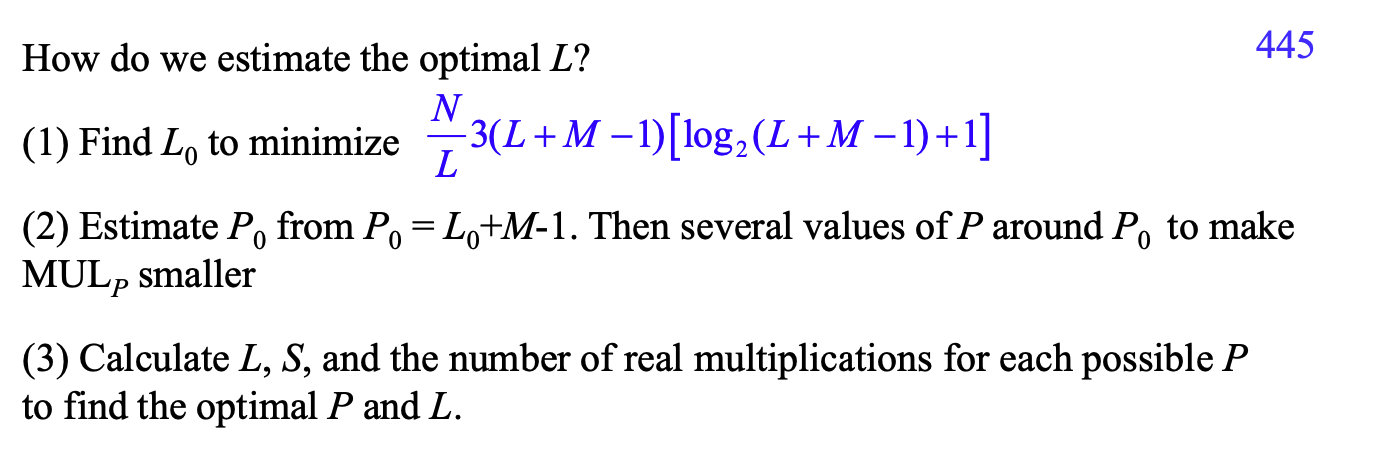
\includegraphics[width=0.8\textwidth]{HW4_img/7_process.png}
\end{figure}

\bigskip

I wrote a python code to implement the above steps, and the code is as follows:

\begin{figure}[H]
    \centering
    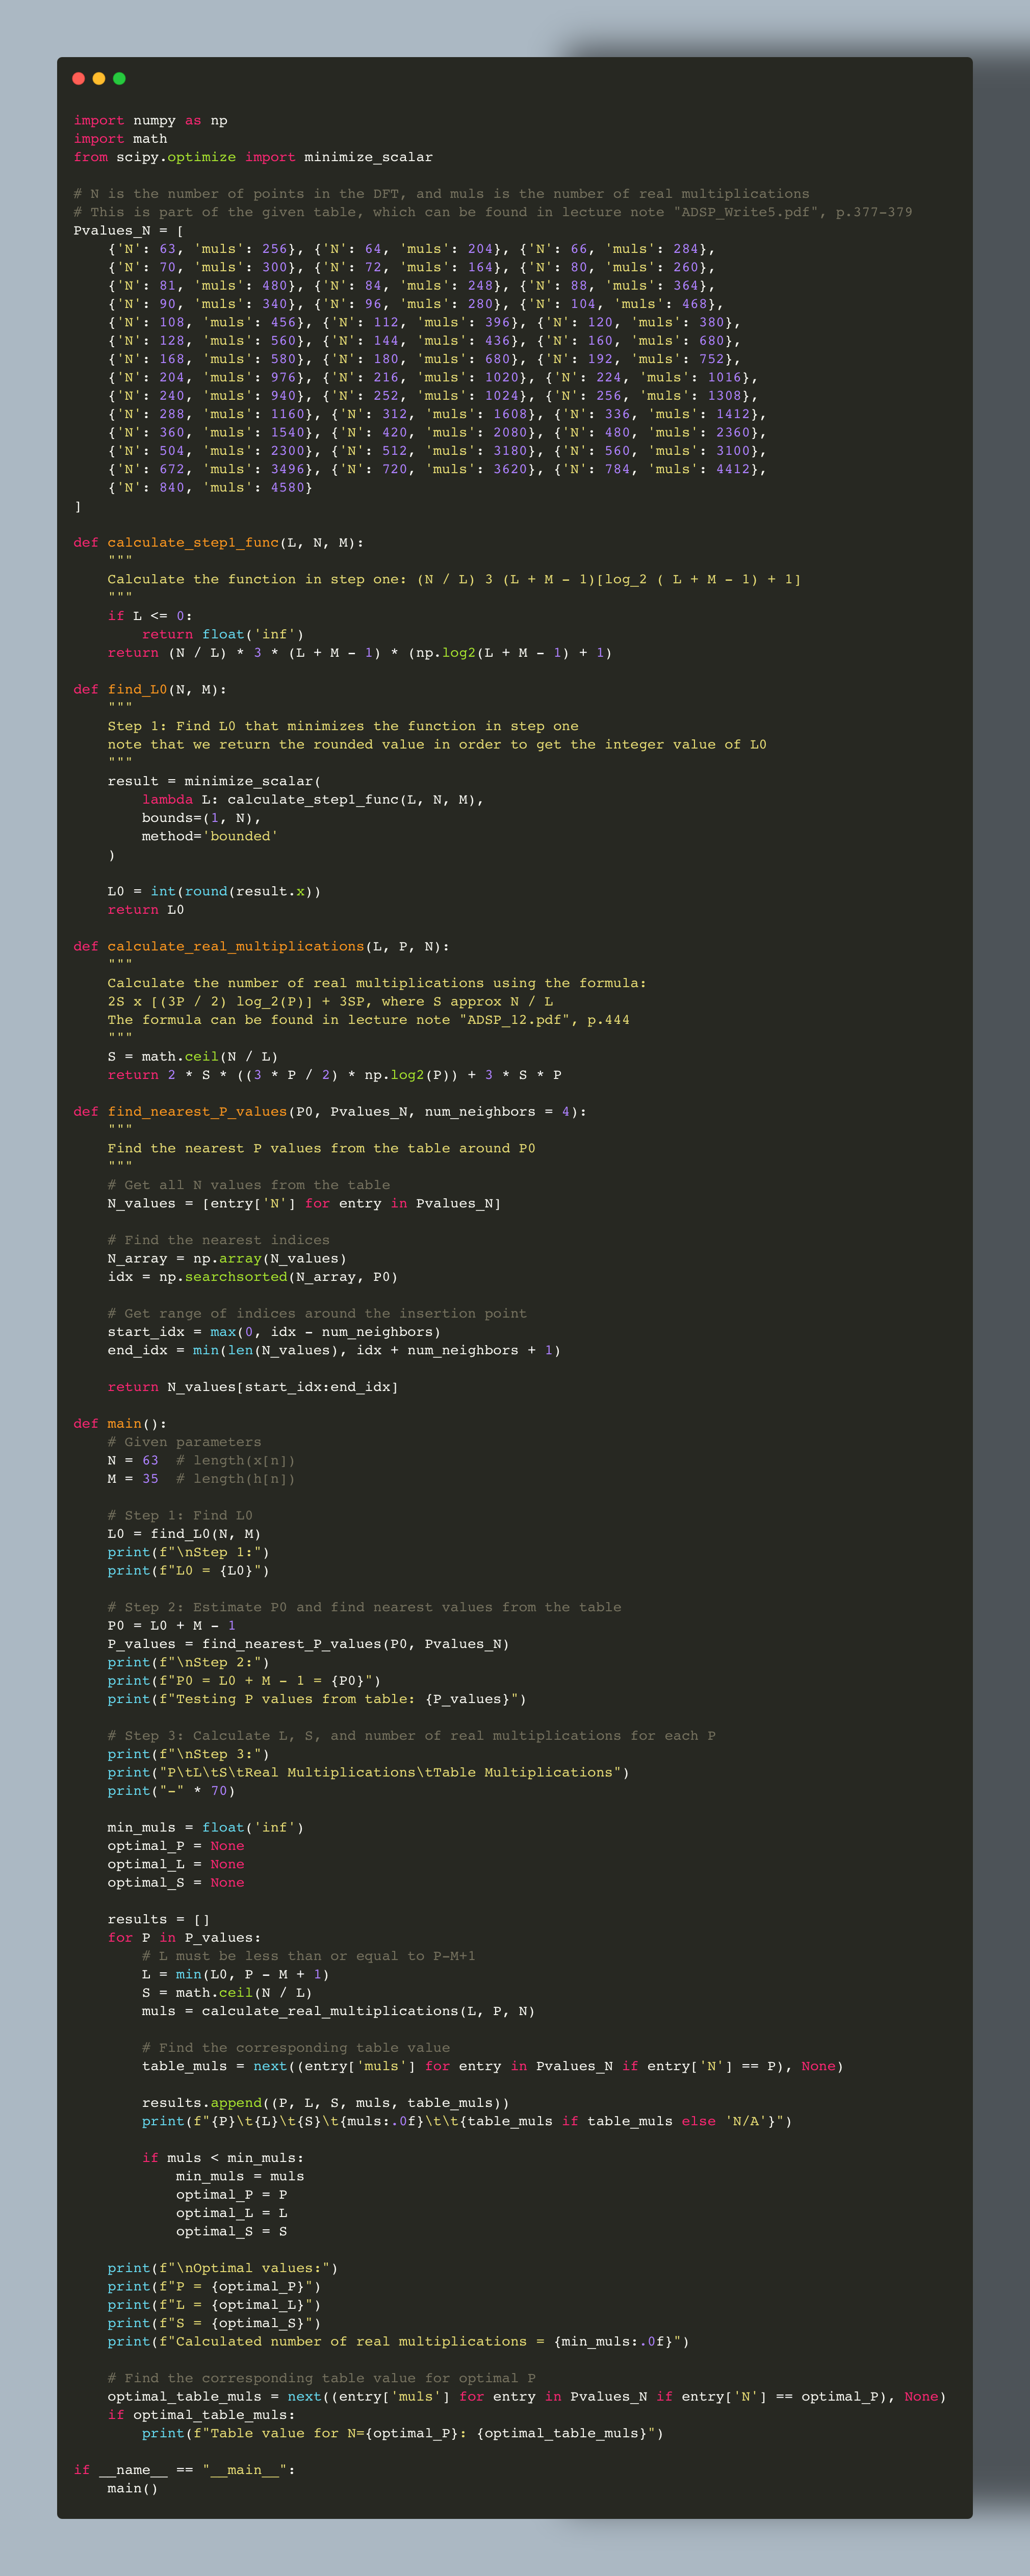
\includegraphics[width=0.7\textwidth]{HW4_img/7_code.png}
\end{figure}

and by running the code, we can get the following result:

\begin{figure}[H]
    \centering
    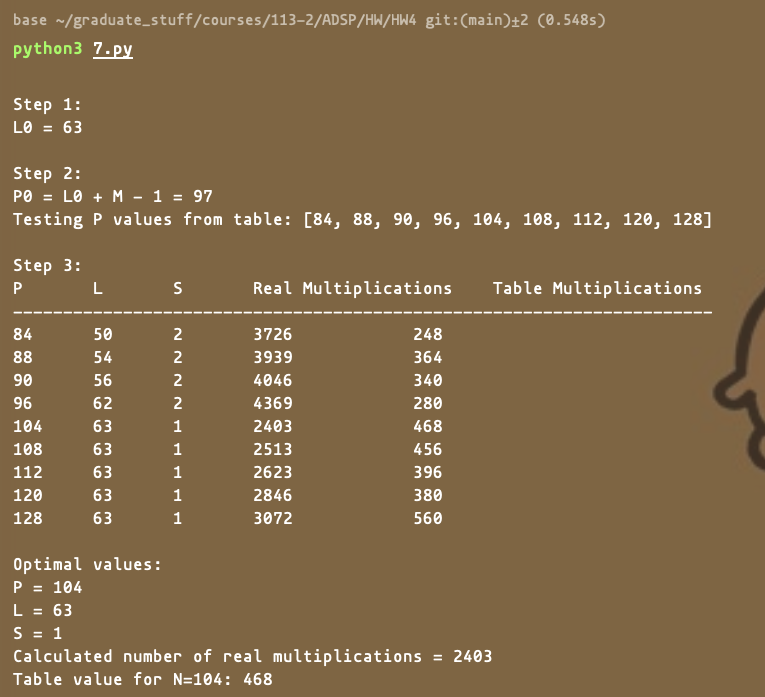
\includegraphics[width=0.7\textwidth]{HW4_img/7_result.png}
\end{figure}

Therefore, we can see that the optimal number of points for the DFT is $P = 104$.
\bigskip

(Since the image might be not that clear, if the original code file is needed, please inform me.)

\section*{(8)}

We're required to determine the number of real multiplications for the following $x$-point DFTs:
\bigskip

Our approach is first decomposing the given $x$-points into factors, 
then use the table in lecture note: "ADSP\_Write5.pdf", p.377-379,
to find the corresponding value of MUL\_x, except the subproblem (c), 
a little modification is needed to deal with $121 = 11^2$. 
\bigskip


\subsection*{(a)}

For $154$ points DFT:

\begin{align*}
    154 = 11 \times 14
\end{align*}

So we have:

\begin{align*}
    &11 \times \text{MUL}_{14} + 14 \times \text{MUL}_{11} \\
    = \ & 11 \times 32 + 14 \times 40 \\
    = \ & 912
\end{align*}

\subsection*{(b)}

For $165$ points DFT:

\begin{align*}
    165 = 11 \times 15
\end{align*}

So we have:

\begin{align*}
    &11 \times \text{MUL}_{15} + 15 \times \text{MUL}_{11} \\
    = \ & 11 \times 40 + 15 \times 40 \\
    = \ & 1040
\end{align*}

\subsection*{(c)}

For $242$ points DFT:

\begin{align*}
    242 = 2 \times 11^2
\end{align*}

So we have:

\begin{align*}
    & 2 \times \text{MUL}_{121} + 121 \times \text{MUL}_{2} \\
    = \ & 2 \times \text{MUL}_{121} + 121 \times 0 \\
    = \ & 2 \times (11 \times \text{MUL}_{11} + 11 \times \text{MUL}_{11} + 3 \times 10 \times 10) \\
    = \ & 2 \times (11 \times 40 + 11 \times 40 + 300) \\
    = \ & 2 \times 1180 \\
    = \ & 2360
\end{align*}


\end{document}